\documentclass{article}

% Language setting
% Replace `english' with e.g. `spanish' to change the document language
\usepackage[english]{babel}

% Set page size and margins
% Replace `letterpaper' with `a4paper' for UK/EU standard size
\usepackage[letterpaper,top=2cm,bottom=2cm,left=3cm,right=3cm,marginparwidth=1.75cm]{geometry}

% Useful packages
\usepackage{amsmath}
\usepackage{amssymb}
\usepackage{graphicx}
\usepackage{float}
\usepackage{tabularx}
\PassOptionsToPackage{hyphens}{url}\usepackage[colorlinks=true, allcolors=blue]{hyperref}
\usepackage{booktabs} % Unused
\usepackage{blindtext} %usued
\usepackage{url}
\usepackage{multicol}
\usepackage{titling}
\usepackage{indentfirst}
 \geometry{
 a4paper,
 left=1in,
 right=1in,
 top=1in,
 bottom=1in,
 }
\usepackage{caption}
\usepackage{titlesec}
\usepackage{fvextra}
\usepackage{breqn}

\renewcommand\maketitlehooka{\null\mbox{}\vfill}
\renewcommand\maketitlehookd{\vfill\null}

\newcommand{\twitter}{$\mathbb{X}$ (formerly Twitter)}
\newcommand{\tweets}{tweets}
\newcommand{\tweet}{tweet}

\begin{document}

\begin{titlepage}
    \centering
    \vspace*{1in}

    {\Huge \textbf{Tweeting Emotions: Decoding Sentiment in 140 Characters}}\\
    \vspace{0.5in}
    {\huge Final Report \\}
    \vspace{0.5in}
    {\huge Edward Wang \\}
    \vspace{0.25in}
    {\huge Fall 2024}

    \vfill
\end{titlepage}


% \newpage

% \tableofcontents

% \newpage

\begin{multicols}{2}

\begin{abstract}
Sentimental analysis of social media data, particularly Twitter, has become a popular method for gauging public opinion. This study explores sentiment analysis using the Sentiment140 dataset, focusing on extracting insights from \tweets\ for improving business strategies. We compared traditional machine learning models (Naive Bayes, Logistic Regression) with deep learning models (RNN with LSTM). Data preprocessing involved handling internet slang, text normalization, and lemmatization with part-of-speech tagging to boost accuracy. Logistic Regression reached an F1 score of 0.81, while RNN with LSTM achieved 0.82, showing deep learning's edge in sentiment analysis. However, logistic regression provides fast deployment and computational efficiency, making it ideal for quick to market scenarios. Challenges included handling sarcasm and long training times for some models. Future work aims to implement advanced models like BERT and enhance the preprocessing pipeline.
\end{abstract}

\section{Introduction}

Since its inception in 2003, the popularity of social media has surged over 20-times in the past two decades \cite{kemp2024}. Currently, more than two-thirds of adults in the US engage with social networking sites, with an astonishing 90\% participation rate from young adults aged 18 to 29 \cite{perrin2015}. Social media serves as a dynamic platform for users to express their feelings and opinions on a wide array of topic. This ranges from critiques of the latest blockbuster films to in-depth discussions about character development in literature, or even sharing adorable moments of a newborn hippo in Thailand.

Among the various forms of social media, microblogging has gained particular traction. This format "allow users to exchange small elements of content such as short sentences, individual images, or video links" \cite{kaplan2010}. For example, \twitter\ had more than a quarter of a billion daily active users in 2019, with a notable 10\% growth in 2020 \cite{oberlo2024}. The increasing engagement on these platforms highlights their significance as a medium for both personal expression and community interaction.

As social media continues to grow, companies are increasingly eager to tap into this vast reservoir of user-generated content. The insights from analyzing social media data can provide invaluable information about public perception and brand image. With 500 million \tweets\ sent each day in 2022 \cite{sayce2019}, \twitter\ offers a rich source of real-time feedback from consumers. Businesses aim to mine this data to gain a deeper understanding of their audience's views and preferences.

Sentiment analysis, also known as opinion mining, plays a key role in processing unstructured data through Natural Language Processing (NLP) to identify emotional tone of the text \cite{wankhade2022}. By analyzing \tweets\ related to a particular company's product or services, business can uncover trends, gauge customer satisfaction, and identify areas for improvement or expansion. Sentiment analysis enables companies to monitor their public image effectively and engage with their customers. This ultimately helps improve both brand loyalty and marketing strategies. 


\section{Problem Statement}

The objective of this analysis is to identify the most effective models for Natural Language Processing (NLP), with a particular focus on sentiment analysis of online text. This study will utilize various \tweets\ from \twitter, where the contents of each post will be classified into positive or negative sentiments. By analyzing these \tweets, we hope to enhance the understanding of how sentiment analysis can help drive business strategies and improve customer engagement in an increasingly digital world. 


\section{Data Source}

The data source for this analysis is the Stanford Sentiment140 Dataset \cite{go2009twitter}, which contains 1.6 million \tweets\ extracted from \twitter \;API. An example format of a \tweet, created using a fake \tweet\ website \cite{typefully2024}, can be seen in Figure \ref{fig:sample_tweet}. This dataset was collected in 2009 which was an era where posts were limited to 140 characters. This restriction has since been increased to 280 characters. Although the original dataset is no longer hosted by Stanford, it remains accessible through Kaggle \cite{kazanova_sentiment140} and Hugging Face.

\begin{figure}[H]
\centering

\includegraphics[width=1.0\linewidth, ]{tweet-preview.png}
\captionof{figure}{Example of a Tweet}
\label{fig:sample_tweet}
\end{figure}

The dataset consists of five primary components: the ID of the \tweet, the \tweet's posted date, the username of the person who sent it, the content of the \tweet, and the sentiment of the \tweet\ itself classified as either positive or negative. Users can tag other users by including their handles (@), and utilize hashtags (\#) to highlight keywords or topics relevant to their message \cite{metricool2024}.

\section{Proposed Methodology}

\subsection{Data Cleaning}  

In this dataset, \tweets\ often exhibit typical attributes found in online social media. Typical attributes include user mentions, hyperlinks, emojis, abbreviations, and slang \cite{inproceedings}. The \tweets\ may also contain informal language, spelling errors, and special characters \cite{DBLP:journals/corr/DhingraZFMC16}. While some spelling variations may be errors, others are intentionally stylized for emphasis, which is known as netspeak. For instance, posts might feature elongated words such as "heyyyyy", "i gotta get up eeeeaaarrrrlllyyyyyyyy", or substituting words like "that" with "dat" \cite{thangaraj2015influence}. 

The data cleaning process will be broken into three parts. The first part focuses on elements specific to \twitter. This involves the removal of user mentions and hyperlinks to streamline the data for analysis. The second part addresses standardizing netspeak. In this step, we will standardize abbreviations, correct common spelling variations, and normalize informal language to ensure consistency across the dataset. The third part involves optimizing the text for natural language processing (NLP). This includes tasks such as tokenization, lowercasing, and the removal of stopwords, special characters or other irrelevant elements that may reduce the accuracy of our models.

\subsection{Usernames and Hyperlinks}   

All social media platforms distinguish their users with a username. To prevent specific usernames from influencing sentiment analysis, it is essential to eliminate mentions (e.g., @User123). For instance, a user like @PositiveQuoteDaily, who consistently shares positive content, could inadvertently bias the model towards associating this username with positive sentiment. 

Starting with the username, cleaning can be done using regular expressions (Regex) to identify the "@" character that indicates a mention. Usernames on \twitter\ are constrained to no more than 15 characters and must contain only alphanumeric characters, with the exception of underscores \cite{XUsernameRules}. 

Hyperlinks, on the other hand, are more complex. They generally follow specific patterns, starting with "www", "http://", or "https://". Since \twitter\ is a microblogging platform, hyperlinks are often designed to be clicked immediately. Thus, they tend to follow a standardized format and can be easily identified and removed. 

\subsection{Standardizing Netspeak}   

The meaning of words tends to shift both online \cite{LeriqueRoth2018} and in everyday conversations \cite{Liberman2012}. This can complicate the standardization process. We begin by expanding contracted words back into their full form. This allows our model to focus on each individual word rather than the contraction itself. While this is straightforward for cases like "she'll" into "she will", other cases are more complex. For instance, distinguishing between possession and contraction, as in "it's" versus "its", can be challenging. A more difficult example is differentiating between "the cat's toy" and "that's their toy", using python code, as they both end with "t".

As mentioned above, we need to handle posts that feature netspeak. Regex can help identify repeated letters and remove the excess. The approach is to replace any sequence of three or more repeated letters with just two. This would address cases like "heyyyy" or "hhhhhiiiiii", without impacting naturally occurring double-letter words like "ball" or "butter". While there are rare instances of words with more than two repeated letters, such as "hostessship", these occurrences are infrequent and can be handled separately. Cases like "that" and "dat" are not handled in this cleaning process due to time constraints. Addressing such variations would require an extensive mapping file to account for all possible informal language variations. 

\subsection{NLP Preprocessing}   

Preprocessing our text plays a crucial role in building any NLP model \cite{kannan2014preprocessing}. We begin with basic cleaning steps. HTML tags, also known as character entity references, are often used to escape special characters on websites \cite{raggett1997html}. For example, "\&amp;" represents the "\&" sign. Using the html package, we can quickly replace these tags with their original ASCII form. Accented characters are also replaced with their standard ASCII equivalents. Finally, the entire text is converted to lowercase to eliminate case-sensitive discrepancies.

To enhance the quality of the data, it is crucial to remove stopwords \cite{ghag2015}. These are defined as commonly occurring words in natural language that contribute little to the overall meaning.  Stopwords include articles, conjunctions, prepositions, pronouns, and frequently used verbs. For example, some popular ones are: "the", "and", "is", "in", "to" \cite{sarica2021}.

Since words can take various forms based on tense, techniques such as stemming or lemmatization are necessary to reduce them to their root forms \cite{stanford_nlp_stemming_lemmatization}. While both methods aim to reduce words to their base forms, stemming works by simply trimming the start or end of the word, whereas lemmatization considers the word's original meaning. Stemming is computationally simpler than lemmatization, but the latter is generally more accurate \cite{khyani2021interpretation}. Given the significant advances in computing power over the past decade, the computational cost of lemmatization has become negligible. Therefore, we will be using lemmatization in our process.

\section{Modeling}

\subsection{Model Architectures}

The objective of this analysis is to conduct sentiment analysis on online text. A neural network model is well-suited for this task, particularly the Recurrent Neural Network (RNN). RNNs are a type of deep learning architecture designed to handle sequential data, making them especially effective for natural language processing (NLP) and speech recognition tasks \cite{shervine_rnn_cheatsheet}.


One such model is the Long Short-Term Memory (LSTM) network, which excels at capturing long-term dependencies in text sequences \cite{usha2021}. LSTMs are a specific type of RNN designed to address the limitations of traditional RNNs when learning long-term dependencies. They use a set of gates to regulate the flow of information, allowing the network to selectively retain important information in memory \cite{hochreiter1997long}. This makes LSTMs especially well-suited for tasks like sentiment analysis on \tweets, where the meaning of a message often depends on the context provided by preceding words or phrases. Furthermore, Bidirectional LSTMs take this a step further by processing input data in both forward and backward directions. This captures context from both past and future states to improve performance.

Beyond RNNs, exploring other types of neural networks, such as transformers, is essential for tackling more complex NLP tasks. For example, state-of-the-art models like BERT \cite{huggingface_bert}, developed by Google, have led to significant advancements in NLP and set new benchmarks in the field.

Traditional machine learning models can also be used as our dataset represents a binary classification problem. These models could serve as benchmarks to evaluate the performance of the neural networks. Examples of such models include naive Bayes, K-Nearest Neighbor (KNN), logistic regression, and decision tree. A study that performed binary classified hate speech in \tweets, for instance, used similar models \cite{akuma2022}. 

In the example of a decision tree, the text would have to be converted to bag of words or TF-IDF. Bag of words essentially looks at if certain known words are in the text opposed to the location. TF-IDF looks at the term frequency within the text \cite{hacohen2020influence}. 

\subsection{Model Tuning}

Model tuning plays a critical role in optimizing model performance. Each of the models described earlier has hyperparameters that must be adjusted to find the best performing variation. For neural networks, one of the most important hyperparameters is the learning rate which determines the step size at each iteration during training \cite{WU201926}. Other key hyperparameters include batch size, number of layers, dropout rate, and optimizers. The batch size defines how many examples are processed before updating the model, while the number of layers dictates the complexity of the model. The dropout rate randomly drops certain layers during training, which helps reduce overfitting. The choice of optimizer also influences how quickly the model converges. In models like random forest, hyperparameters such as the number of trees, tree depth, and minimum samples per leaf impact the model's performance by controlling its complexity and how it splits the data.

There are three main approaches to selecting hyperparameters for these models. The first is to use the default parameters or manually chosen values. Often this doesn't provide the best possible model. A more systematic approach is to use grid search, which evaluates a predefined set of hyperparameters in a grid-like fashion. However, a study by Bergstra et al. (2012) argues that random search can be more efficient than grid search in certain cases \cite{bergstra2012random}. While we plan to use grid search initially, we may switch to random search if grid search proves to be too time-consuming.

\subsection{Model Metrics}

We aim to split our dataset into an 80/20 ratio, with 80\% used for training and 20\% reserved for testing. Ideally, we would use more than 15\% of the data for testing, as suggested in \cite{google_ml_crash_course}. To determine the best hyperparameters for each model, we will use metrics like accuracy on the training dataset, which will allow us to track the best performance. The testing dataset will then be used to assess the final performance of the model. This is because the testing dataset is new and hasn't been seen before by the model. In addition, we will apply cross-validation to ensure that the model performs optimally and generalizes well across different subsets of the data.

To compare the performance of the various models, we will use the F1 score. The F1 score ranges from 0 to 1, where 0 represents the worst value and 1 represents the best. It combines the precision and recall metrics using the harmonic mean \cite{grandini2020metrics}. This balanced metric allows for a fair comparison across models and ensures that both precision and recall perform well overall. However, it is still important to exercise caution and examine the individual precision and recall values. A model with a high F1 score could still have one metric (i.e., precision or recall) that is much lower than the other, which may indicate an imbalance in performance. 

\section{Analysis and Results}

\subsection{Exploratory Data Analysis}  

Before proceeding with the modeling process, we first examined the dataset. The Sentiment140 dataset is evenly split, with 800,000 \tweets\ in each sentiment label. After applying our data cleaning process in python, approximately 3,000 \tweets\ were removed as they consisted solely of direct mentions of other users without providing any meaningful text.

One key decision in our data cleaning process was to avoid removing stopwords. In his article, Aleti argues that indiscriminately removing stopwords can alter the sentiment of the original text \cite{aleti2020stopwords}. He provides the example of the negative sentiment "The product is not good," which, after stopwords are removed, becomes "product good," changing the sentiment to positive. 

When applying lemmatization, some words were not processed correctly. We used part-of-speech tagging to address this issue which improved the lemmatization process. Part-of-speech tags each word as a noun, verb, adjective, or adverb, essentially identifying the grammatical role of each word. With this fix, we were able to ensure that words were lemmatized appropriately based on their context.

The most frequent words in both positive and negative \tweets\ can be observed in Figure \ref{fig:pos_wc} and Figure \ref{fig:neg_wc} respectively. Some words, such as "go", "now", and "will", appear with similar frequency in both the positive and negative word clouds. The positive sentiment word cloud features more terms related to gratitude and love, while the negative sentiment word cloud highlights themes of work and a sense of loss.

\begin{figure}[H]
\centering
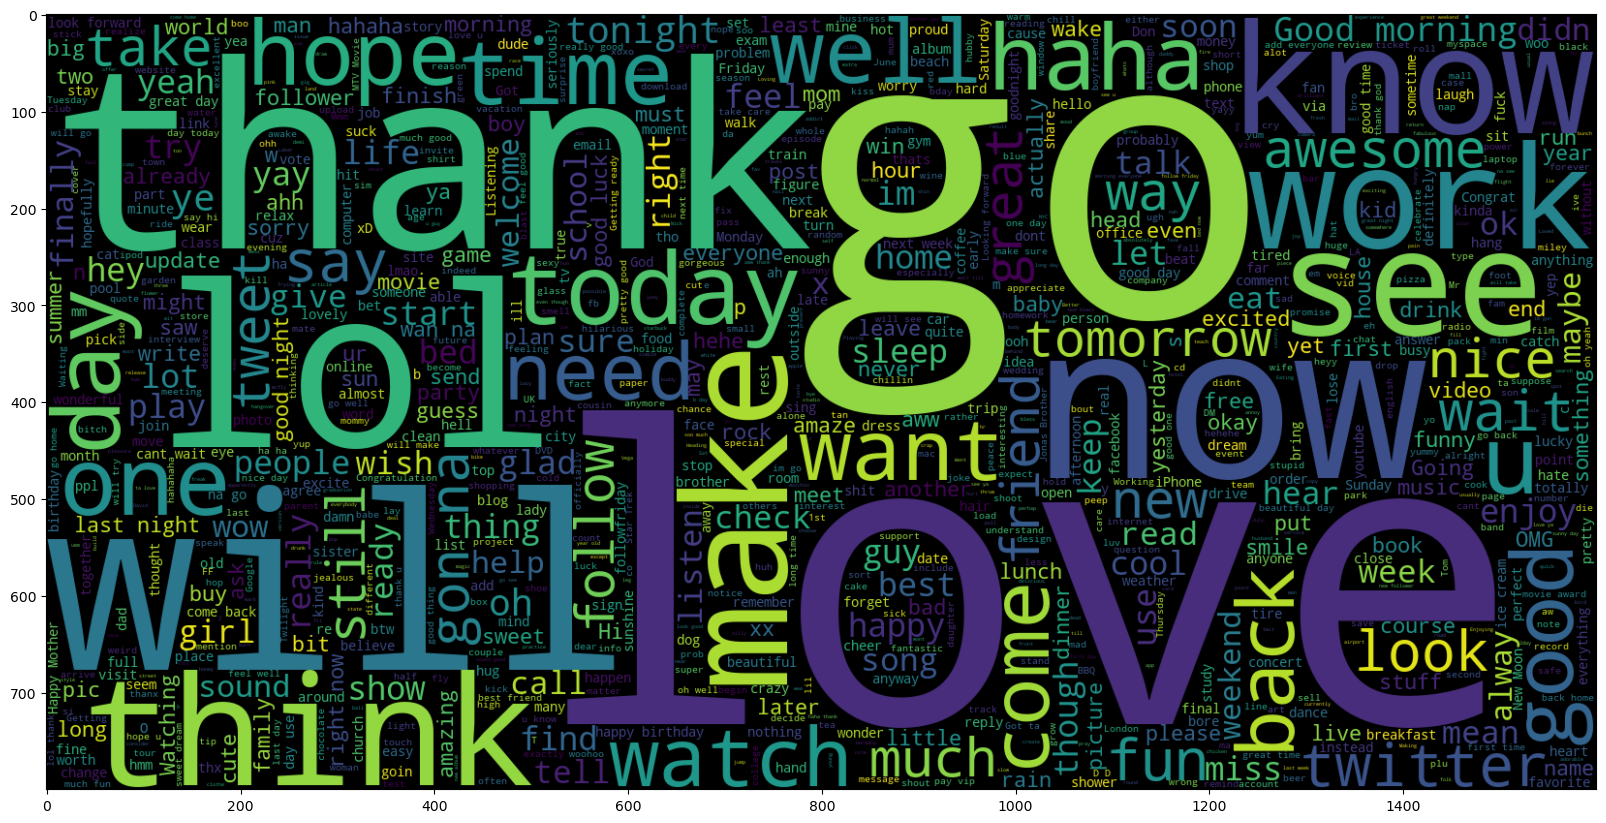
\includegraphics[width=1.0\linewidth, ]{cleaned_wc_positive.png}
\captionof{figure}{Positive Sentiment Word Cloud}
\label{fig:pos_wc}
\end{figure}

\begin{figure}[H]
\centering
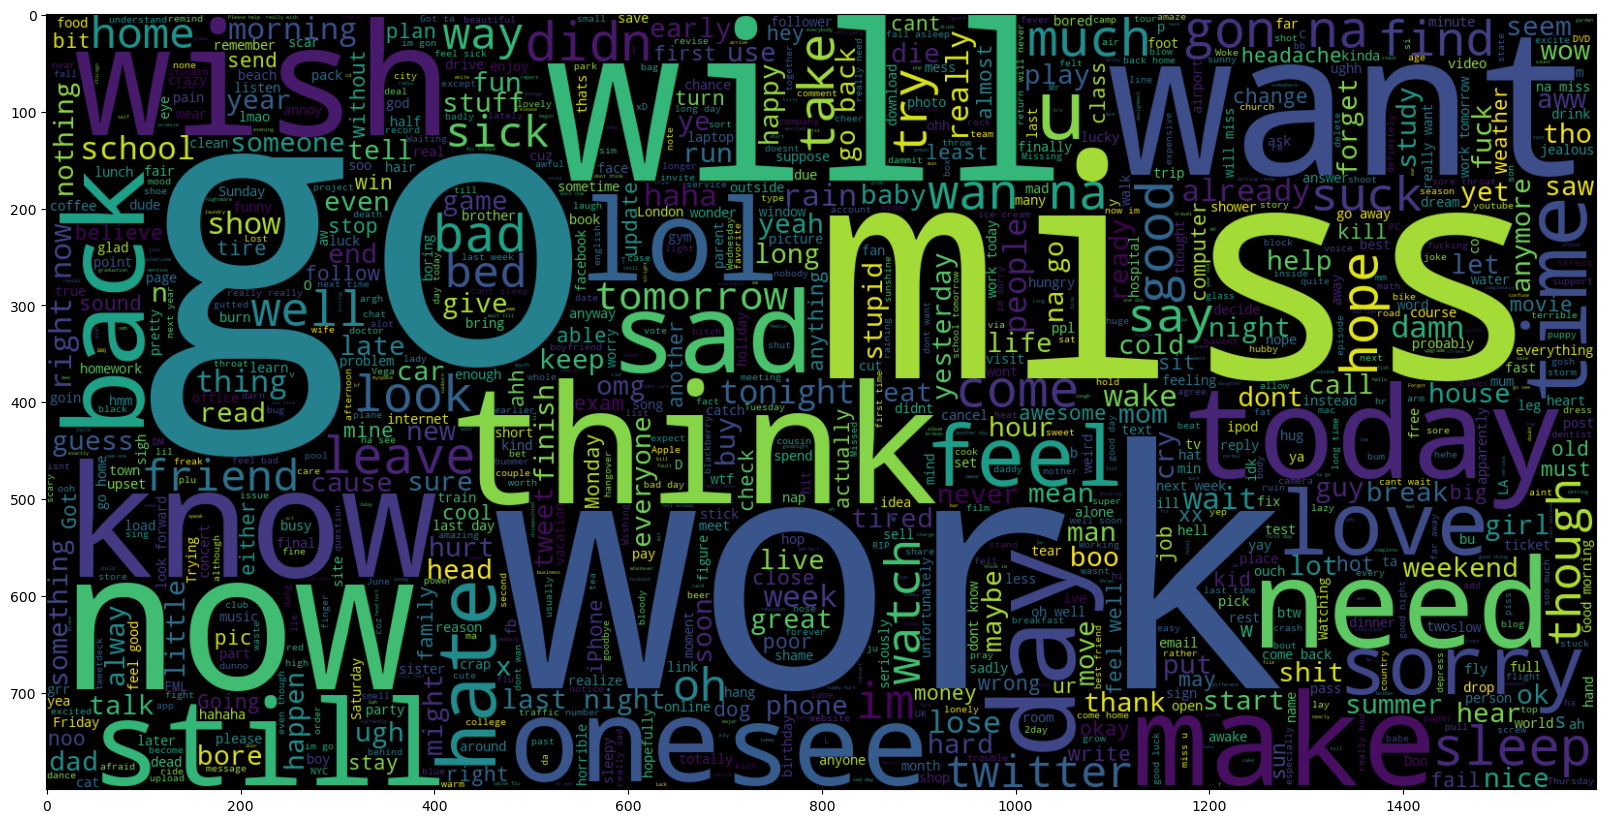
\includegraphics[width=1.0\linewidth, ]{cleaned_wc_negative.png}
\captionof{figure}{Negative Sentiment Word Cloud}
\label{fig:neg_wc}
\end{figure}

\subsection{Modeling Results}

The simpler models, naive Bayes and logistic regression, were trained first. The dataset was vectorized using the TfidfVectorizer package in Python, with a maximum of 10,000 features and included both uni-grams and bi-grams. The corresponding hyperparameters are listed in Table \ref{tab:hyperparameters}. 

\begin{center}
\small 
\begin{tabular}{ll}  
\toprule
\textbf{Model} & \textbf{Parameters} \\ 
\midrule
Bernoulli Naive Bayes & \(\alpha: [0.1{-}1.0]\) \\ 
Logistic Regression & \(C: [10^{-3}{-}10^3]\) \\ 
   & \(penalty: ['l2']\) \\
\bottomrule
\end{tabular}
\captionof{table}{Hyperparameters for Random Search} 
\label{tab:hyperparameters}
\end{center}

\begin{table*}[t]
\small
\centering
\begin{tabular}{lccccc}
\toprule
\textbf{Model}                    & \textbf{F1 Score} & \textbf{Accuracy} & \textbf{TP} & \textbf{TN} & \textbf{Confusion Matrix}                                             \\ 
\midrule
Bernoulli Naive Bayes             & 0.77                     & 0.77                     & 126,594                    & 119,824                    & \([ [119824, 40263], [32683, 126594] ]\)                                \\ 
Logistic Regression               & 0.81                     & 0.81                     & 130,303                    & 127,417                    & \([ [127417, 32670], [28974, 130303] ]\)                                \\ 
Bernoulli Naive Bayes (RS)        & 0.78                     & 0.77                     & 126,583                    & 119,853                    & \([ [119853, 40234], [32694, 126583] ]\)                                \\ 
Logistic Regression (RS)          & 0.81                     & 0.81                     & 130,303                    & 127,417                    & \([ [127417, 32670], [28974, 130303] ]\)                                \\ 
RNN with LSTM                     & 0.82                     & 0.82                     & 132,752                    & 130,583                    & \([ [130583, 26952], [20853, 132752] ]\)                              \\ 
\bottomrule
\end{tabular}
\caption{Model Performance}
\label{tab:model_performance}
\end{table*}

For naive Bayes, random search identified 0.1 as the optimal alpha value, which improved the F1 score from 0.77 (using default parameters) to 0.78. For logistic regression, random search found that an inverse regularization strength of 1 provided the best performance, which coincidentally matched the default setting. The F1 score for logistic regression was 0.81. Both models were evaluated using 100-fold cross-validation to reduce the risk of overfitting. Finally, the trained models were saved using the joblib package, enabling them to be easily imported for future use.

The Random Forest model took an unexpectedly long time to train. On a Ryzen 3600 CPU, released in 2019, it took approximately 3 minutes per tree. With 100 trees and 5-fold cross-validation, training the model would have taken over a full day. This was before any hyperparameter tuning which would have increased the runtime even further. One attempt to reduce training time was to decrease the number of input features from 10,000 to 1,000, and reduce the number of trees from 100 to 20. This cut the training time to about 1 minute per tree. Unfortunately this would have still taken hours to train. Google Colab was also tested, but discrepancies in the results and limited time for root cause analysis led to it being discarded. Given the delays in text processing, the Random Forest model was ultimately removed from the project.

\begin{figure}[H]
\centering
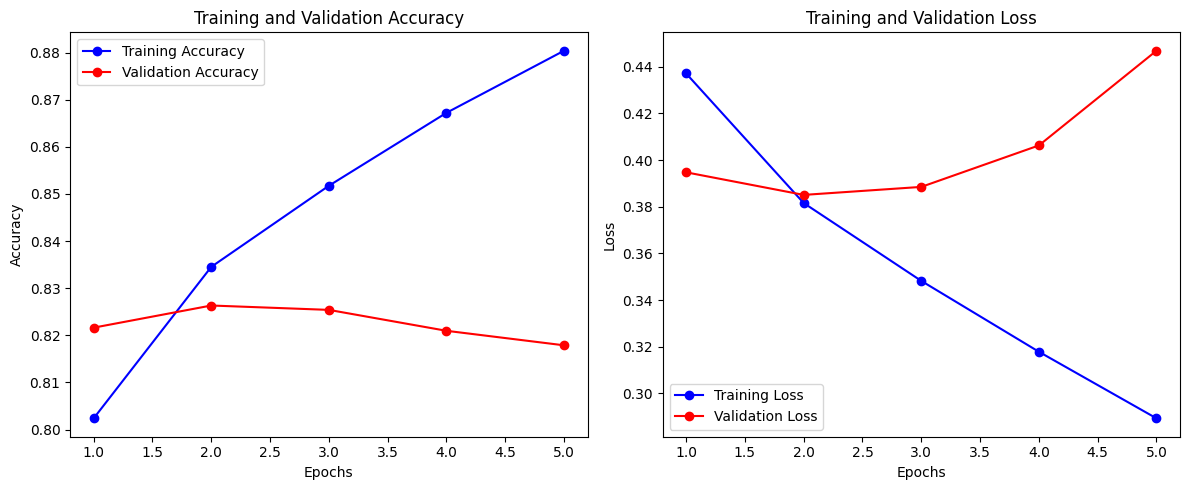
\includegraphics[width=1.0\linewidth, ]{RNN_training_history.png}
\captionof{figure}{RNN Training and Validation \\ \footnotesize Note: A larger version can be found in the appendix.}
\label{fig:rnn_training}
\end{figure}


The Recurrent Neural Network (RNN) model was implemented using the TensorFlow package in Python. The architecture consists of six layers: one embedding layer, one LSTM layer, two dense layers, and two dropout layers (See Appendix). Early stopping was used to prevent overfitting. As shown in Figure \ref{fig:rnn_training}, the model achieved its best performance at epoch 2, where the validation accuracy was highest and the validation loss was lowest. After epoch 2, the validation loss began to rise while the accuracy fell. This suggests the model had reached its optimal performance. The RNN achieved the best overall performance with an F1 score of 0.82 as summarized in Table \ref{tab:model_performance}.

\section{Conclusion}

In this study, we explored sentiment classification using the Sentiment140 dataset. We compared multiple models, including simpler methods like Naive Bayes and Logistic Regression, as well as the more complex Recurrent Neural Network (RNN). After preprocessing the data and addressing issues with lemmatization, we trained the models while leveraging hyperparameter tuning and cross-validation. The models were evaluated using F1 scores, and overfitting was prevented through techniques such as early stopping and random search for optimal parameters.

Our results demonstrate that the simpler models, Naive Bayes and Logistic Regression, performed adequately with F1 scores of 0.78 and 0.81 respectively. These were fast and easy to implement, but failed to fully capture the sequential nature of text. The RNN model achieved the best overall performance, with an F1 score of 0.82. This highlights the effectiveness of using deep learning techniques for sentiment analysis, particularly in capturing the nuances of language.

Given time constraints in a competitive business environment, logistic regression offers a practical solution. It provides solid performance with faster training times compared to complex models like neural networks, allowing companies to deploy models quickly. This speed enables businesses to stay ahead of competitors by iterating faster and responding more swiftly to market demands, without sacrificing too much accuracy.

For future work, several areas can be explored. One limitation in this study was the handling of sarcastic comments, which were not addressed in the modeling process. Another direction is revisiting the Random Forest model to overcome its limitations and improve its performance. It would also be valuable to experiment with the Bag of Words method as an alternative feature extraction technique. We woudl want to compare its results with those obtained using TF-IDF. Although BERT was considered for this study, there was not enough time to fully implement and compare its performance. Exploring BERT and other advanced models in future work could offer significant improvements in sentiment classification.

\subsection{Lessons we have learned}

Several important lessons were learned during this process. The most significant one was the failure to train a random forest model within the allotted time. In hindsight, this issue likely stemmed from the decision to retain stop words, which increased the number of input features and ultimately slowed the model's training down to a crawl.

Another key lesson was that lemmatization alone was not sufficient. Words can have multiple meanings depending on context which cans issues further down the line. To make the lemmatization process more effective, it became clear that incorporating parts of speech was essential for achieving the desired results. Additionally, text preprocessing turned out to be more complex than initally anticipated.

Finally, narrowing the project scope or adding more team members would have greatly helped in meeting all the original objectives within the planned timeline.

\bibliographystyle{plainurl}
\bibliography{sample}

\end{multicols}

\pagebreak

\appendix
\section{Larger Versions of Figures}

\begin{figure}[H]
\centering

\includegraphics[width=1.0\linewidth, ]{tweet-preview.png}
\captionof{figure}{Tweet format}
\end{figure}

\begin{figure}[H]
\centering
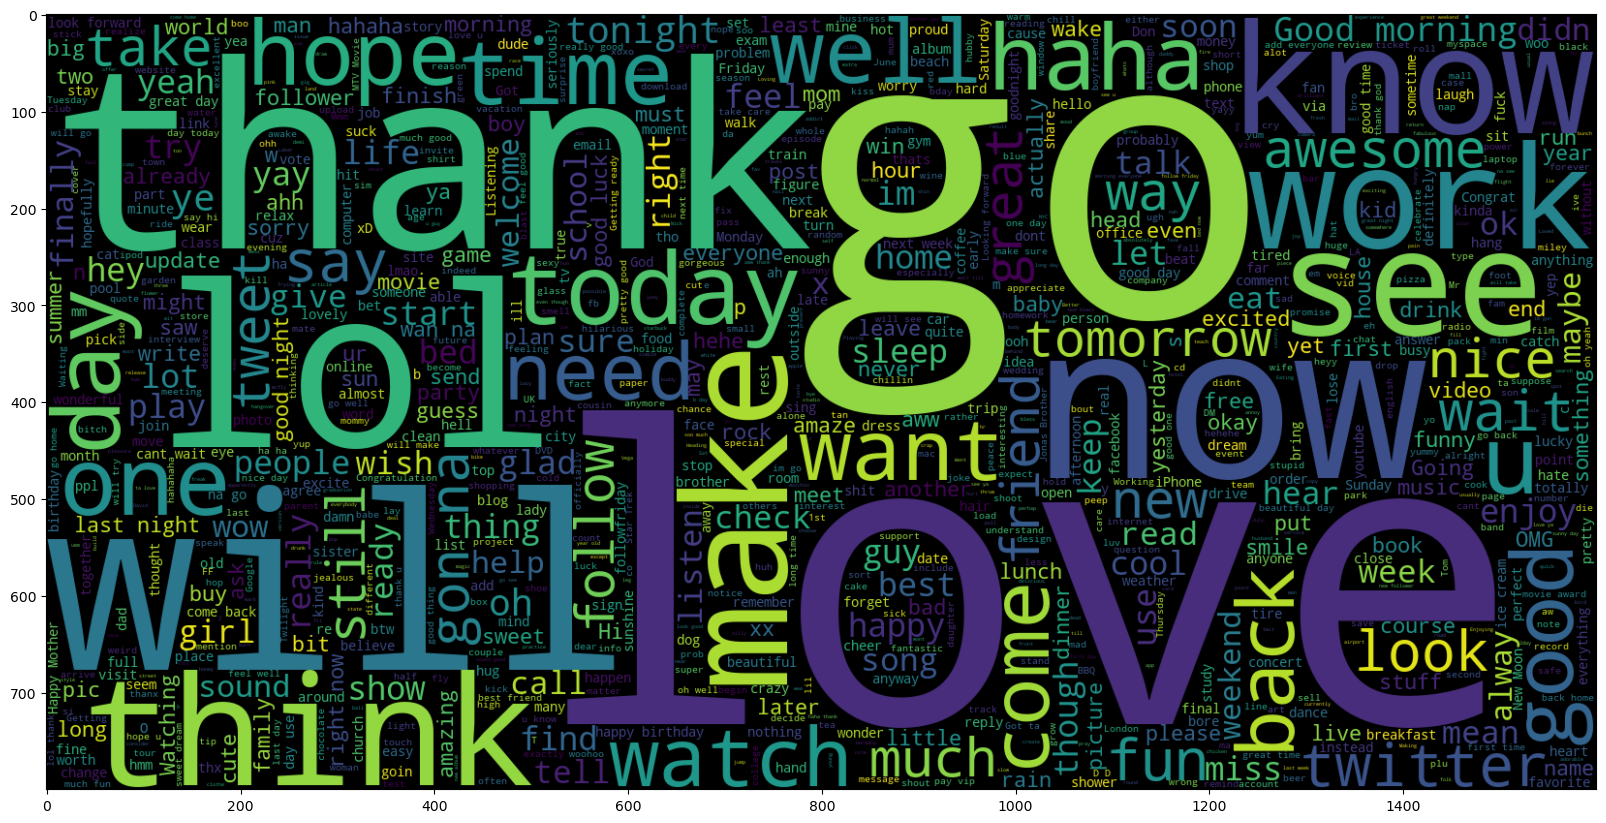
\includegraphics[width=1.0\linewidth, ]{cleaned_wc_positive.png}
\captionof{figure}{Positive Sentiment Word Cloud}
\end{figure}

\begin{figure}[H]
\centering
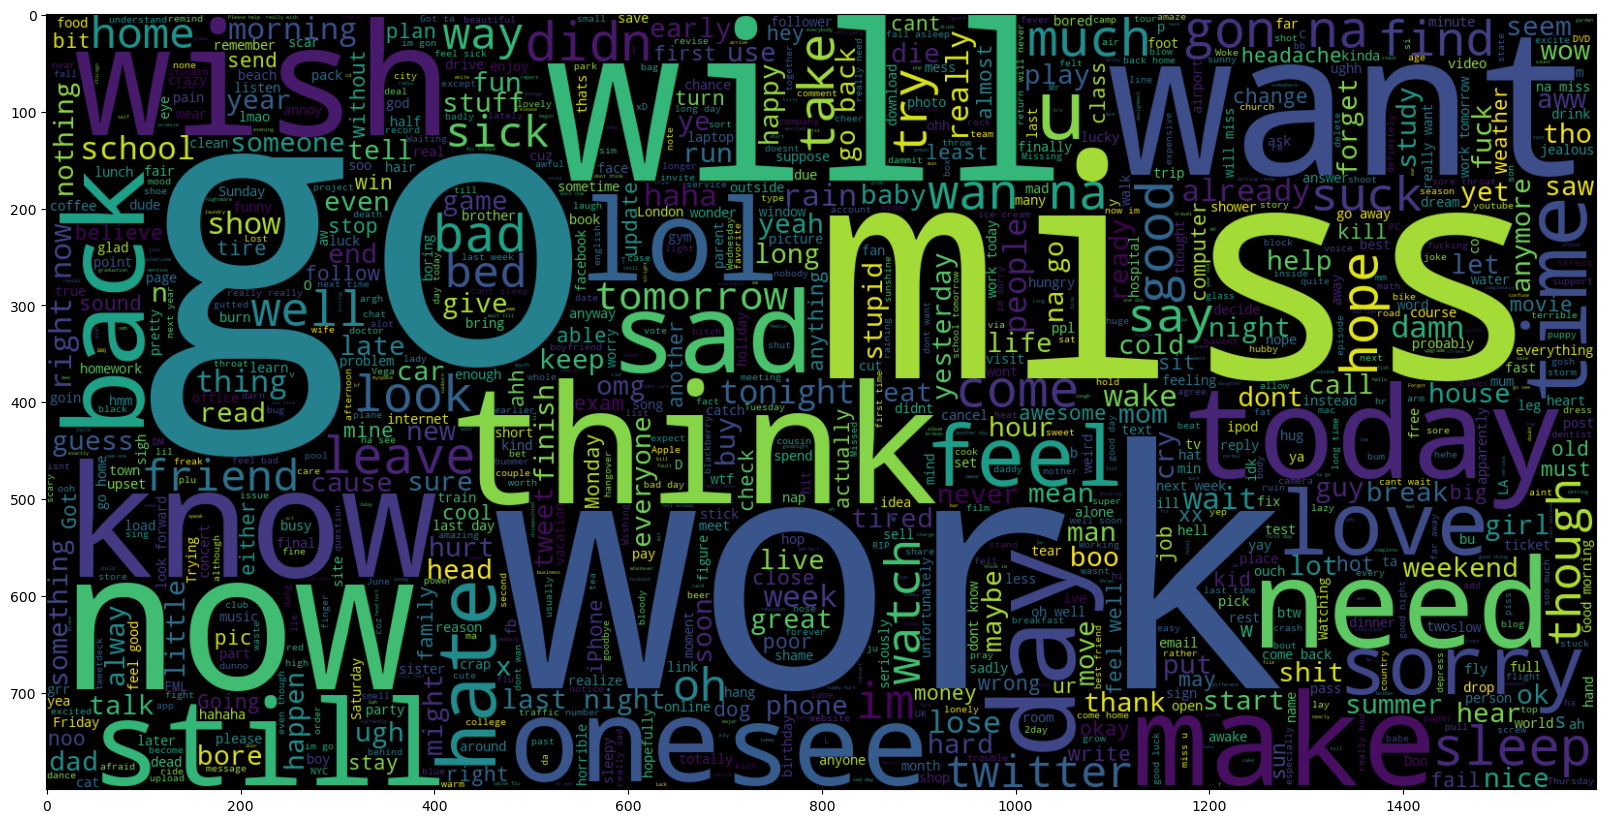
\includegraphics[width=1.0\linewidth, ]{cleaned_wc_negative.png}
\captionof{figure}{Negative Sentiment Word Cloud}
\end{figure}

\begin{figure}[H]
\centering
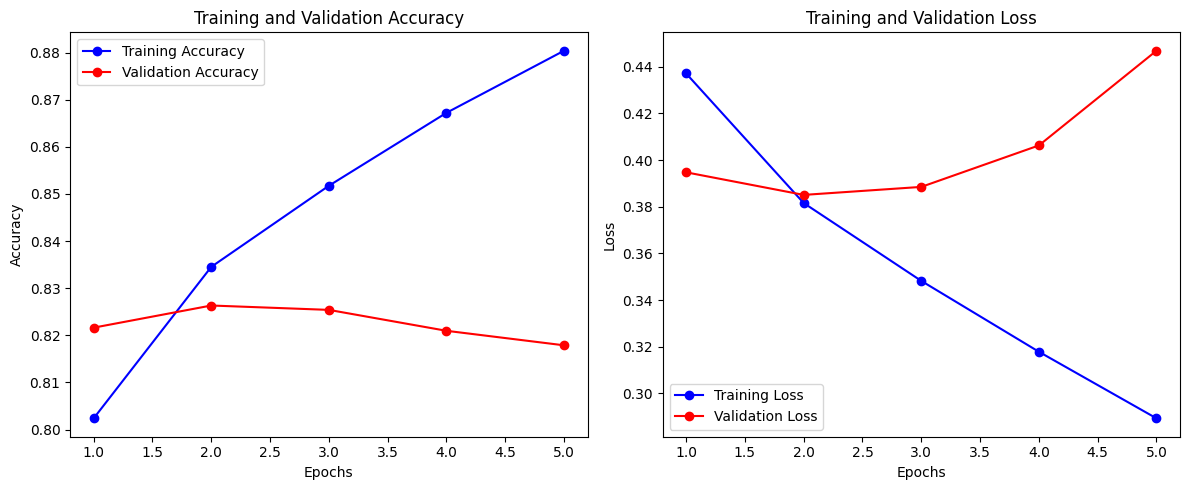
\includegraphics[width=1.0\linewidth, ]{RNN_training_history.png}
\captionof{figure}{RNN Training and Validation}
\label{fig:rnn_training}
\end{figure}

\section{Additional Figures}

\begin{figure}[H]
\centering
\includegraphics[width=1.0\linewidth, ]{data_example.png}
\captionof{figure}{Sample Dataset}
\end{figure}

\begin{figure}[H]
\centering
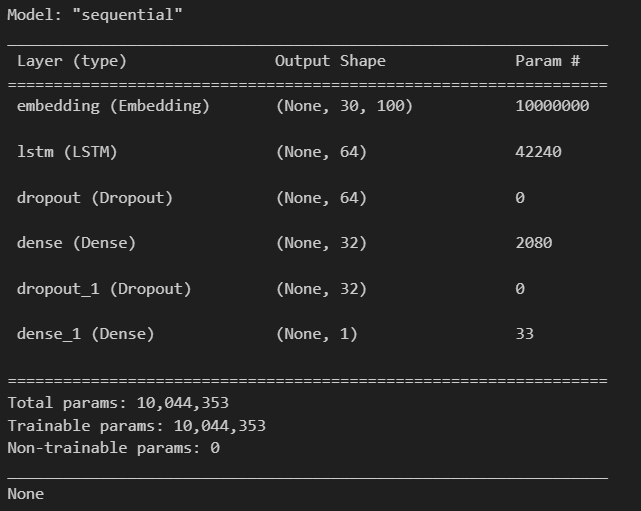
\includegraphics[width=0.75\linewidth, ]{rnn_layers.png}
\captionof{figure}{RNN Layers}
\end{figure}

\begin{figure}[H]
\centering
\includegraphics[width=0.75\linewidth, ]{sample_prediction.png}
\captionof{figure}{Model Predictions on Sample Tweets}
\end{figure}

\end{document}
